\documentclass{ltxdockit}
\usepackage{dtklogos,csquotes,graphicx}

\newcommand\pkgversion{0.2}

\titlepage{%
  title={The showhyphens package},
  subtitle={Show all possible hyphenation points},
  url={(none yet)},
  author={Patrick Gundlach},
  email={patrick@gundla.ch},
  revision={\pkgversion},
  date={\today}}

\begin{document}
\printtitlepage
\tableofcontents

\section{Documentation}

When you load the package \texttt{showhyphens} in your \LuaLaTeX\ document, \LaTeX\ will show all possible hyphenation points. This
package requires you to process the document with \LuaLaTeX.

\begin{verbatim}
\documentclass{article}
\usepackage{showhyphens}

\begin{document}
A wonderful serenity has taken
possession of my entire soul, like these
sweet mornings of spring which I enjoy
with my whole heart. I am alone, and
feel the charm of existence in this
spot, which was created for the bliss of
souls like mine. I am so happy, my dear
friend, so absorbed in the exquisite
sense of mere tranquil existence, that I
neglect my talents. I should be
incapable of drawing a single stroke at
the present moment; and yet I feel that
I never was a greater artist than now.
\end{document}
\end{verbatim}

yields \vspace{5mm}

\noindent 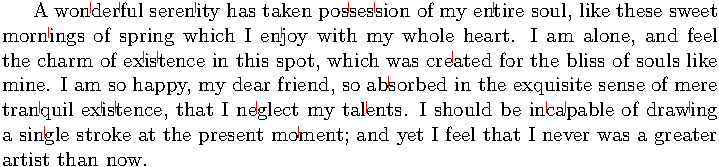
\includegraphics{showhyphens-sample}

\section{Options}

\begin{optionlist}
\legitem{blue}{Shows hyphenation marker in blue, instead of red.}
\end{optionlist}


\section{Changes}

\begin{changelog}
\begin{release}{0.2}{2012-10-25}
  \item New option \enquote{blue}, thanks go to Herbert Voß.

\end{release}
\end{changelog}

\section{Copying}

Copyright 2011 Patrick Gundlach (patrick@gundla.ch), licensed under the MIT license. See the style for details.


\end{document}
